\documentclass[../ZF_Wing.tex]{subfiles}

\begin{document}





\textbf{Begriff: } Verstehen (Analyse) und Befriedigen (Aktivitäten, 4P-Mix) von Märkten und von Kundenbedürfnissen um die unternehmerische Ziele zu erreichen. \\

\begin{figure}[H]
\centering
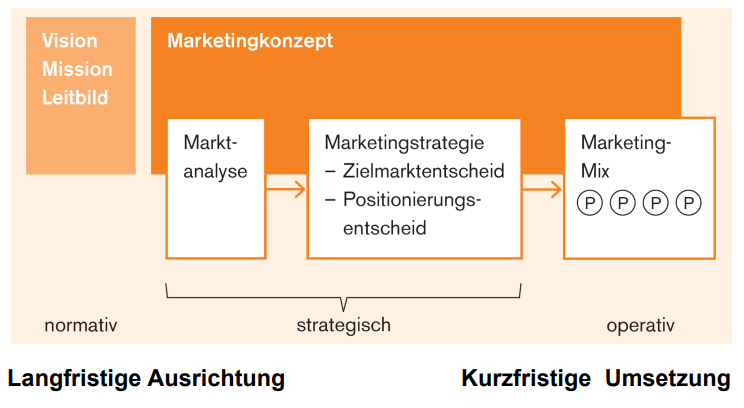
\includegraphics[width=0.3\textwidth]{Resources/Image/BegriffMarketing.png}
\caption{\label{fig:BegriffMarketing}BegriffMarketing.}
\end{figure}

\title{Absätzmärkte}

\begin{figure}[H]
\centering
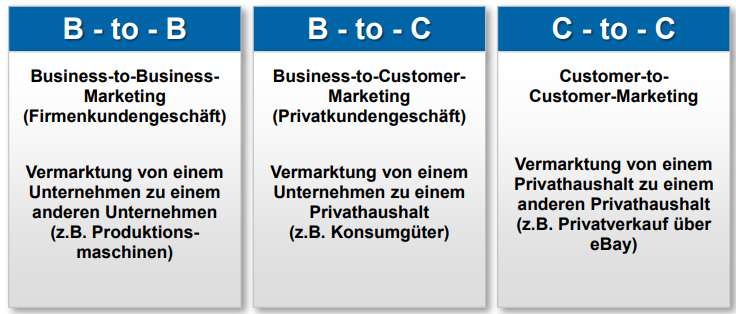
\includegraphics[width=0.3\textwidth]{Resources/Image/Absatzmarkt.png}
\caption{\label{fig:BegriffMarketing}BegriffMarketing.}
\end{figure}


\subsection{Marktanalyse}


														


\begin{tabular}{|l|l|l|}
\hline 
\textbf{Marktforschung} & \textbf{ Ziel} & {Typische Fragen} \\ 
\hline
\rule[-1ex]{0pt}{2.5ex}  
\textbf{Qualitativ} & Zahlenwerte über den Markt ermitteln & Marktvolumen?Marktanteil eines Unternehmens\\ 
\hline 
\textbf{Quantitativ} & Motive, Verhalten Kunden & Erwartungen, Warum kauft  \\ 
\hline 
\end{tabular} 

\subsubsection{Erhebungsmethoden}


\begin{multicols}{2}

\textbf{Field Research / Primärforschung}
\begin{itemize}
	\item Befragung Personen
	\item Gespräch Branchenexperten
	\item Besuch Veranstaltungen / Messen
	\item Stiller Beobachter
\end{itemize}

\columnbreak
\textbf{Desk Research/ Sekundärforschung}
\begin{itemize}
	\item Wissenschaftliche Publikationen
	\item Unternehmensinformationen
	\item Brancheniformation
	\item Öffentliche Informationen
	\item Sonstige Nachschlagewerke
\end{itemize}


\end{multicols}


\subsubsection{Marktgrössen}
\begin{figure}[H]
\centering
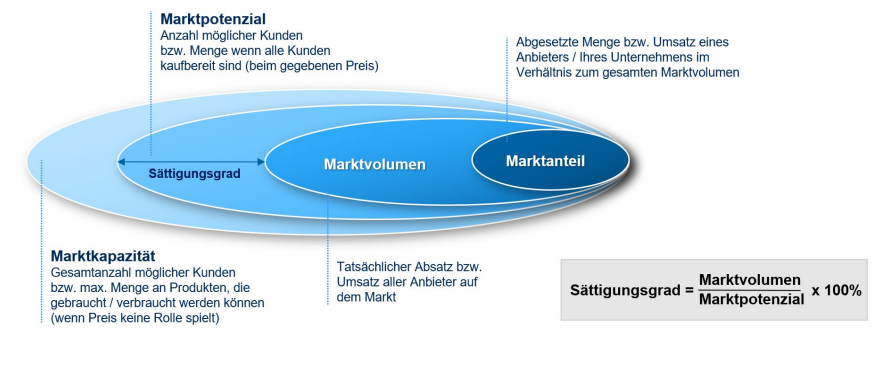
\includegraphics[width=0.3\textwidth]{Resources/Image/Marktgroessen.png}
\caption{\label{fig:BegriffMarketing}Marktgroessen .}
\end{figure}

\textbf{Marktsegmentierung}\\

\textbf{Definition: } Aufteilung des Gesamtmarktes in homogene Käufergruppen nach bestimmten Kriterien

\begin{multicols}{3}

\begin{figure}[H]
\centering
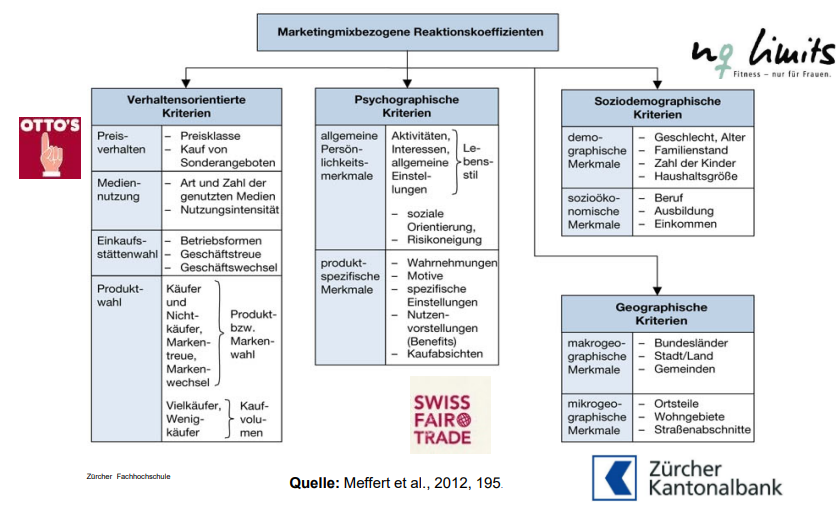
\includegraphics[width=0.3\textwidth]{Resources/Image/ModellSegmentierung.png}
\caption{\label{fig:ModellSegmentierung}ModellSegmentierung.}
\end{figure}


\columnbreak
\begin{figure}[H]
\centering
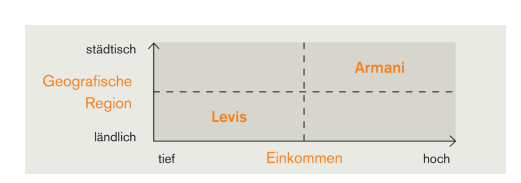
\includegraphics[width=0.3\textwidth]{Resources/Image/AbgrenzungGeographisch.png}
\caption{\label{fig:BegriffMarketing}AbgrenzungGeographisch.}
\end{figure}

\columnbreak
\begin{figure}[H]
\centering
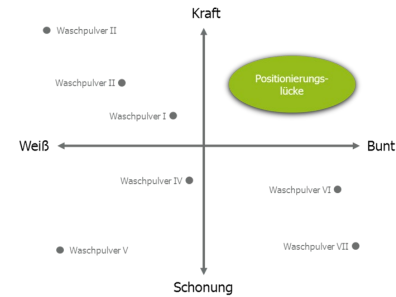
\includegraphics[width=0.3\textwidth]{Resources/Image/AbgrenzungEigenschaften.png}
\caption{\label{fig:AbgrenzungEigenschaften}AbgrenzungEigenschaften.}
\end{figure}



\end{multicols}

\subsection{Marketing 4P-Mix}


\begin{multicols}{4}
\textcolor {orange} {\textbf{Product}}
\begin{itemize}
	\item Absatzprogramm / Sortiment
	\item Produkteigenschaften
	\item Verpackung
	\item Serviceleistungen
	\item Garantieleistungen
\end{itemize}


\columnbreak
\textcolor {orange} {\textbf{Price}}
\begin{itemize}
	\item Preisbestimmung
	\item Preisstrategie
	\item Konditionen
\end{itemize}

\columnbreak
\textcolor {orange} {\textbf{Place}}
\begin{itemize}
	\item Absatzwege
	\item Transportmittel
\end{itemize}

\columnbreak
\textcolor {orange} {\textbf{Promotion}}
\begin{itemize}
	\item Werbung
	\item Öffentlichkeitsarbeit
	\item Sponsoring
\end{itemize}


\end{multicols}



\subsubsection{Produktgestaltung}

\begin{multicols}{3}
\textcolor {orange} {\textbf{Gestaltung des Produktkerns (Grundnutzen)}}
\begin{itemize}
	\item Grösse
	\item Gewicht
	\item Material
	\item technische Leistung
	\item Bedienungsfreundlichkeit
\end{itemize}


\columnbreak
\textcolor {orange} {\textbf{Gestaltung des Produktäusseren(Zusatznutzen)}}
\begin{itemize}
	\item Design (Form, Farbe)
	\item Verpackung
	\item Markierung
\end{itemize}

\columnbreak
\textcolor {orange} {\textbf{Zusatzleisungen (Kundenservice)zum Produkt}}
\begin{itemize}
	\item Beratung
	\item Schulung
	\item Zustellung
	\item Installation
	\item Reparatur und Garantiedienst
\end{itemize}




\end{multicols}


\title{Verpackung Funktionen}

\begin{multicols}{2}
\textcolor {orange} {\textbf{Technische Funktionen}}
\begin{itemize}
	\item Transportfunktionen
	\item Lagerfunktionen
	\item Schutzfunktionen
\end{itemize}


\columnbreak
\textcolor {orange} {\textbf{Kommunikative Funktionen}}

\begin{itemize}
	\item Informationsfunktion
	\item Werbemittelfunktion
	
\end{itemize}

\end{multicols}



\subsubsection{Preisstrategie}

\paragraph{Preishöhe: } Je höher der Preis, desto höher ist bei einer bestimmten Absatzmenge der Umsatz des Unternehmens.\\

\paragraph{Absatzmenge: } Der Preis beeinfluss die absetzbare Menge des Gutes. In der Regel sinkt die Absatzmenge eines Gutes bei steigendem Preis.

\title{3 Ansätze der Preisfestsetzung}

\begin{multicols}{4}
\textcolor {orange} {\textbf{Nachfrageorientierung}}
\begin{itemize}
	\item Ausgangspunkt
	\begin{itemize}
		\item Zahlungsbereitschaft der Kunden
	\end{itemize}
\end{itemize}

\columnbreak

\textcolor {orange} {\textbf{Kostenorientierung}}
\begin{itemize}
	\item Ausgangspunkt
	\begin{itemize}
		\item Kosten des Produkts für das Unternehmen
	\end{itemize}
\end{itemize}

\columnbreak

\textcolor {orange} {\textbf{Wettbewerbsorientierung}}
\begin{itemize}
	\item Ausgangspunkt
	\begin{itemize}
		\item Preise der Konkurrenz
	\end{itemize}
\end{itemize}
	
\columnbreak
\begin{figure}[H]
\centering
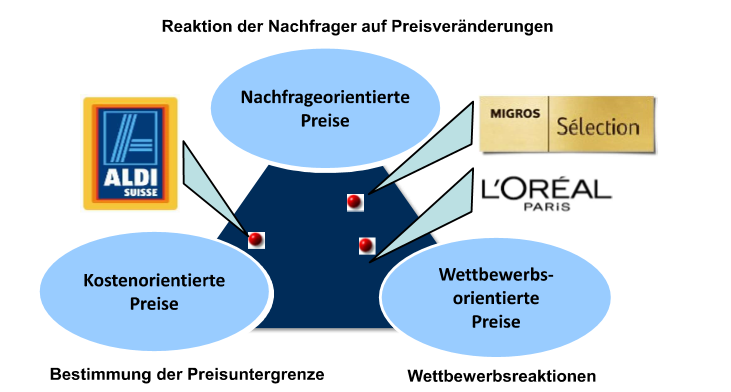
\includegraphics[width=0.3\textwidth]{Resources/Image/ReaktionNachfrager.png}
\caption{\label{fig:ReaktionNachfrager}ReaktionNachfrager.}
\end{figure}

\end{multicols}


\title{Die Break-Even-Analyse}

\paragraph{Defintion: } Bewertungsmodell zur Ermittlung der Absatzmenge, die erforderlich ist, um die Gewinnschwelle zu erreichen.

\begin{figure}[H]
\centering
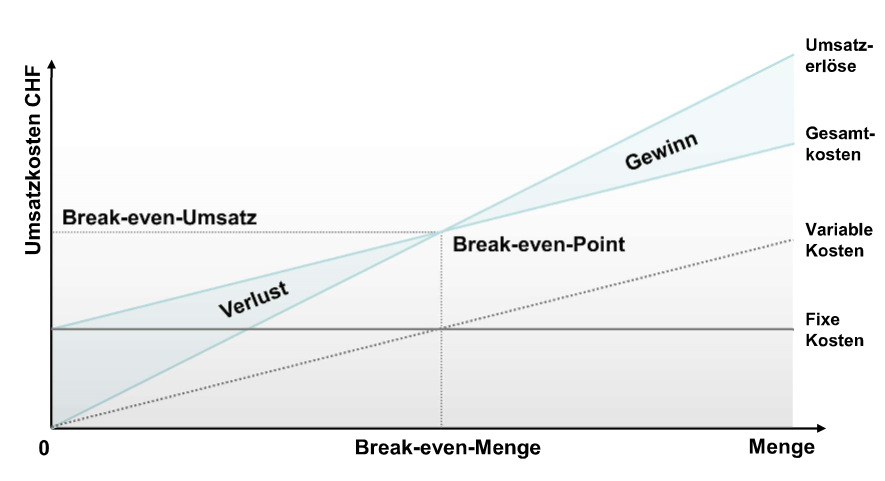
\includegraphics[width=0.3\textwidth]{Resources/Image/Break-Even-Analyse.png}
\caption{\label{fig:BreakEvenAnalyse}BreakEvenAnalyse.}
\end{figure}


\title{\textbf{Typische preispolitische Massnahmen}}

\begin{table} [H]

\begin{tabular}{l}

\colorbox{pink!30}{\textbf{Zeitliche Preisdifferenzierung} }

\\\hline
Tag-/Nachttarif (telefonieren)\\
 Billigere Hotelzimmer in Nebensaison\\
 Normal- und Ausverkaufspreise\\
\end{tabular}
\end{table}


\begin{table} [H]

\begin{tabular}{l}

\colorbox{pink!30}{\textbf{Räumliche Preisdifferenzierung} }

\\\hline
In- und Auslandpreise (Medikamente)\\

\end{tabular}
\end{table}


\begin{table} [H]

\begin{tabular}{l}

\colorbox{pink!30}{\textbf{Preisdifferenzierung Käuferschichten} }

\\\hline
Studententarife\\
Verbilligung für Aktionäre\\
\end{tabular}
\end{table}

\begin{table} [H]

\begin{tabular}{l}

\colorbox{pink!30}{\textbf{Preisdifferenzierung nach Abnahmemenge} }

\\\hline
Mengenrabatte\\
Treueprämien\\
Bundling\\
\end{tabular}
\end{table}

\begin{table} [H]

\begin{tabular}{l}

\colorbox{pink!30}{\textbf{Zeitliche Preisdifferenzierung} }

\\\hline
Tag-/Nachttarif (telefonieren)\\
 Billigere Hotelzimmer in Nebensaison\\
 Normal- und Ausverkaufspreise\\
\end{tabular}
\end{table}




\begin{table} [H]

\begin{tabular}{l}

\colorbox{pink!30}{\textbf{Strategie der hohen Einführungspreise -> \textcolor {red}{Skimming}} }

\\\hline
Computer\\
Video- und Audiogeräte\\

\end{tabular}
\end{table}


\begin{table} [H]

\begin{tabular}{l}

\colorbox{pink!30}{\textbf{Strategie der niedrigen Einführungspreise -> \textcolor {red}{Penetration}}}

\\\hline
Waschmittel\\
Getränke\\
Lebensmittel\\

\end{tabular}
\end{table}

\begin{table} [H]

\begin{tabular}{l}

\colorbox{pink!30}{\textbf{Gratis-Angebot und Freemium}}

\\\hline
Netzwerke\\
Online-Spiele\\
Apps\\
\end{tabular}
\end{table}

\begin{table} [H]

\begin{tabular}{l}

\colorbox{pink!30}{\textbf{Preisdifferenzierung nach Nutzungsverhalten}}

\\\hline
Software\\
Online/Printmedien\\
Apps\\

\end{tabular}
\end{table}


\begin{table} [H]

\begin{tabular}{l}

\colorbox{pink!30}{\textbf{Beachtung psychologischer Effekte / Grenzen}}

\\\hline
19.90 statt 20.--\\
9.95 statt 10.--\\

\end{tabular}
\end{table}



\begin{figure}[H]
\centering
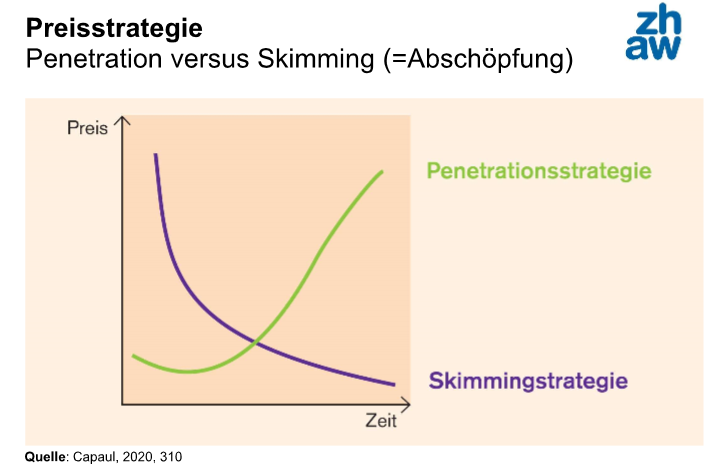
\includegraphics[width=0.3\textwidth]{Resources/Image/PenetrationvsSkimming.png}
\caption{\label{fig:PenetrationvsSkimming}PenetrationvsSkimming.}
\end{figure}


\title{\textbf{Die Elastizität der Nachfrage \\}}

\textbf{Preiselastische Nachfrage: } Nachfrage sinkt  mit steigendem Preis. \\

\textbf{Preisunelastische Nachfrage: } Nachfrage sinkt kaum mit steigendem Pris. \\

\textbf{Inverse Nachfrage: } Nachfrage steigt mit steigendem Preis.


\begin{figure}[H]
\centering
\includegraphics[width=0.3\textwidth]{Resources/Image/Elastizität.png}
\caption{\label{fig:Elastizität}Elastizität.}
\end{figure}



















































\end{document}